\begin{refsection}

\section{Metallic Fuel in Sodium (FRED-M-Na)}
\label{sec:fred_m_na}

FRED-M-Na extends the FRED platform for U-Pu-Zr ternary metallic fuel rods in sodium-cooled fast reactors.  The same core heat conduction and stress-strain equations (Section~\ref{sec:thermo_mech}) are used with HT-9 ferritic-martensitic cladding and additional physics specific to metallic fuel:

\begin{itemize}
\item \textbf{Ternary U-Pu-Zr phase diagram}: phase state (alpha, beta, gamma, delta) affects thermal properties.
\item \textbf{Thermal conductivity with Na infiltration and irradiation}: sodium filling of open pores increases effective conductivity; burnup further modifies it.
\item \textbf{Zirconium redistribution}: Zr migrates from the hot fuel centre to the cooler periphery under steep temperature gradients, changing composition and phase radially.
\item \textbf{Sodium infiltration}: sodium from the coolant infiltrates open fuel porosity after the fuel contacts the cladding.
\item \textbf{Fuel swelling (solid FP)}: solid fission product swelling narrows the gap on a per-at\% burnup basis.
\item \textbf{Fission gas release (Karahan empirical model)}: the cumulative release fraction $f_r$ is a burnup-saturation function calibrated to EBR-II data \cite{karahan2009}:
\begin{equation*}
  f_r(B_\mathrm{FIMA}) = 0.8\!\left(1 - e^{-100\,B_\mathrm{FIMA}/1.8}\right),
  \qquad \bar{B}_\mathrm{FIMA} \geq 8\times10^{-3},
\end{equation*}
where $100\,B_\mathrm{FIMA}$ converts to atomic percent and the condition enforces a rod-average burnup threshold of $0.8\,\mathrm{at\%}$ before any gas is released.  The fraction saturates near 80\,\% by ${\sim}10\,\mathrm{at\%}$; released Xe/Kr dilute the gap gas and raise plenum pressure.
\item \textbf{Cladding wastage}: lanthanides from fission products diffuse into HT-9, consuming cladding material.
\end{itemize}

All correlations are ported from the Fortran reference code \texttt{FRED\_M\_OCT24.SRC} \cite{timpanoFredM} following Karahan (2009) \cite{karahan2009}.

% -------------------------------------
\subsection{Time Integration: Fixed-Step Backward Euler with Explicit Irradiation-Physics Coupling}
\label{sec:mna_time_integration}
% -------------------------------------

FRED-ROD and FRED-OX advance the full DAE state vector $\mathbf{y}$ through SUNDIALS IDA's adaptive-step BDF corrector (Section~\ref{sec:sundials}). FRED-M-Na uses its own fixed-step driver instead, inherited from the structure of legacy \texttt{Baseir.for} and retained because attempts to drive the same physics through SUNDIALS IDA proved numerically fragile. The fission-gas swelling/contact transition produces a near-discontinuous change in residual character that causes IDA's adaptive step-size control to reduce $h$ to unacceptably small values, eventually exhausting the corrector's ability to converge, while the legacy fixed-step approach passes through the same regime without issue.  

Therefore, no IDA calls: \texttt{IDACreate}, \texttt{IDAInit}, \texttt{IDASolve}, or \texttt{IDAReInit} calls exist anywhere in the FRED-M-Na application. The SUNDIALS \texttt{N\_Vector} type is retained purely as a plain data buffer so that checkpoint and HDF5-restart machinery from \texttt{FredSolverBase} works without modification.

At each step two numerically distinct update steps are applied in sequence to two disjoint groups of state variables:
\begin{itemize}
\item an \textbf{implicit, backward-Euler} update for the primary thermal/mechanical DAE unknowns (temperatures, stresses and strains, gas pressure, fission-gas generation and release); and
\item an \textbf{explicit, forward-Euler} update for the irradiation-physics accumulators (burnup, GRSIS bubble/gas-release state, Zr redistribution, cladding wastage), evaluated \emph{after} the implicit solve.
\end{itemize}

Algorithm~\ref{alg:mna_timestep} summarises the complete per-step logic.

\begin{algorithm}[H]
\caption{FRED-M-Na: one fixed step $t_n \to t_{n+1} = t_n + \Delta t$}
\label{alg:mna_timestep}
\begin{algorithmic}[1]
  \Statex \textbf{--- Implicit backward-Euler solve ---}
  \For{outer $= 1$ \textbf{to} 60}
    \State Update $f_\mathrm{gen}$, $f_\mathrm{rel}$ by direct substitution
    \For{each axial layer $j = 1,\ldots,N_z$}
      \State Dense Newton solve ($\leq 25$ iters, FD Jacobian):
      \Statex \qquad\qquad solve for $[T_1,\ldots,T_{n_f+n_c},\;
                 \varepsilon^{sw}_i,\; \varepsilon^{cr}_i,\;
                 b,\; \boldsymbol{\sigma}, \boldsymbol{\varepsilon},\; P_\mathrm{gas}]$
      \Statex \qquad\qquad using $\dot{y}_k \approx (y_k - y_k^{(n)})/\Delta t$
                 for ODE rows, $\dot{y}_k = 0$ for AE rows
    \EndFor
    \If{$\|\Delta P_\mathrm{gas}\| < 10^{-6}$ \textbf{and} layer corrections $< 10^{-6}$}
      \State \textbf{break}
    \EndIf
  \EndFor
  \State Accept last current state even if residuals $> 10^{-6}$   (no SUNDIAL's style step-size shrink or retry)
  \Statex
  \Statex \textbf{--- Explicit forward-Euler update (\texttt{afterAcceptedStep}) ---}
  \For{each axial layer $j$}
    \State \textbf{Burnup}: $B_{FIMA,j} \mathrel{+}= \bigl(q_v''' \,/\, (E_{fiss}\,n_{HM})\bigr)\,\Delta t$
    \State \textbf{GRSIS} bubble/gas-release: explicit Euler sub-stepped at
           $\delta t \leq 1000\,\mathrm{s}$
    \State \textbf{Zr redistribution}: explicit Euler flux-difference, 20 sub-steps
    \State \textbf{Cladding wastage}: explicit Euler diffusion, 20 sub-steps
    \State \textbf{Gap state}: evaluate contact regime $\in \{\texttt{open},\; \texttt{soft},\; \texttt{closed}\}$ from updated gap geometry; update residual branch for next step
    \State \textbf{Hard-contact burnup}: on the first transition to \texttt{closed}, record $B_{FIMA,j}^{hard} \gets B_{FIMA,j}$ (used by the sodium-infiltration ramp-down, Eq.~\eqref{eq:sinf})
  \EndFor
  \State Sync updated irradiation state to residual assembler (one-step lag)
\end{algorithmic}
\end{algorithm}

\noindent\textbf{Performance.} A representative 2176-day base-irradiation simulation (\path{examples/fred_m_na/timpano_SAS_benchmark/base_irradiation/}) with $\Delta t = 1\,\mathrm{day}$ completes in approximately 80\,s wall-clock time on a single core.  Further optimisation of the integrator has therefore not been pursued.

\subsubsection{Implicit backward-Euler solve for the primary DAE unknowns}
\label{sec:mna_backward_euler}

At each fixed step from $t_n$ to $t_{n+1} = t_n + \Delta t$, every differential row of the DAE is discretised with the backward-Euler formula:
\begin{equation}
  \dot{y}_k \approx \frac{y_k(t_{n+1}) - y_k(t_n)}{\Delta t},
  \qquad \mathtt{id}_k = 1,
  \label{eq:mna_be}
\end{equation}
while algebraic rows ($\mathtt{id}_k = 0$) are left undifferentiated.  The \texttt{id}-array convention is identical to that passed to IDA by FRED-ROD and FRED-OX, so the per-layer irradiation ODEs ($b$, $\varepsilon^{sw}_i$, $\varepsilon^{cr}_i$) and the mechanical AEs are typed consistently across all three applications.  Unlike IDA, $\Delta t$ is fixed for the whole step --- there is no adaptive step-size control or local-truncation-error test.

The state vector is partitioned into three rod-scalar globals ($f_\mathrm{gen}$, $f_\mathrm{rel}$, $P_\mathrm{gas}$) and per-layer local blocks.  Layers couple only through the three globals, so the step is solved by an outer Picard sweep (Algorithm~\ref{alg:mna_timestep}, lines 1--8):
\begin{enumerate}
\item $f_\mathrm{gen}$ and $f_\mathrm{rel}$ are updated by direct substitution (their defining equations are explicit in those unknowns).
\item $P_\mathrm{gas}$ is solved \emph{jointly} with each layer's Newton block rather than by direct substitution, because its defining equation depends on all layers' current fuel/cladding radii and axial strain.
\item Each layer's block --- temperatures, per-layer irradiation ODEs ($b$, $\varepsilon^{sw}_i$, $\varepsilon^{cr}_i$), and mechanical AEs ($\boldsymbol{\sigma}$, $\boldsymbol{\varepsilon}$), plus the jointly-solved $P_\mathrm{gas}$ --- is solved by a dense Newton iteration (up to 25 steps, finite-difference Jacobian, tolerance $10^{-7}$) via Eq.~\eqref{eq:mna_be}.
\end{enumerate}
The sweep repeats until both the layer-Newton correction and the change in $P_\mathrm{gas}$ between sweeps fall below $10^{-6}$ (relative), capped at 60 outer iterations.  If the cap is reached, the current iterate is accepted as-is with no retry --- matching legacy \texttt{Baseir.for}'s \texttt{niter\,>\,1000 $\to$ goto\,100} escape.  In practice the sweep converges in 2--4 iterations throughout the full 2176-day benchmark, so this escape is never exercised.

\subsubsection{Explicit forward-Euler update for irradiation physics}
\label{sec:mna_forward_euler}

After the implicit solve has been accepted, \texttt{FredMNaSolver::afterAcceptedStep} advances the irradiation-physics accumulators using explicit (forward) Euler:
\begin{equation}
  X(t_{n+1}) = X(t_n) + \dot{X}\bigl(t_n,\,\mathbf{y}(t_n)\bigr)\,\Delta t,
  \label{eq:mna_fwd_euler}
\end{equation}
i.e.\ rates are evaluated at the already-accepted start-of-step state and not solved implicitly.  The four updated quantities are:
\begin{itemize}
\item \textbf{Burnup} ($B_{FIMA,j}$ per layer): $B_{FIMA,j} \mathrel{+}= (q_v''' / E_{fiss}\,n_{HM})\,\Delta t$.
\item \textbf{GRSIS bubble/gas-release state} (Section~\ref{sec:grsis}): the seven per-node concentrations ($c_{gfm}$, $c_{gb1}$, $c_{gb2}$, $c_{gb31}$, $c_{gb32}$, $c_{ggen}$, $c_{grel}$) are advanced as $X \mathrel{+}= \dot X\,\Delta t$, a direct port of legacy \texttt{GRSIS\_metalfuel.for}, which itself uses unguarded explicit Euler.  Because the legacy driver only called this routine with $\Delta t \approx 1000\,\mathrm{s}$, the call is internally sub-stepped to $\delta t \leq 1000\,\mathrm{s}$ to keep the explicit scheme in the stability regime the model was calibrated for.
\item \textbf{Zirconium redistribution} (Section~\ref{sec:zrdist}): the thermomigration diffusion equation~\eqref{eq:zrdist} is discretised by a conservative radial flux difference and advanced by forward Euler,
    \begin{equation}
      c_{Zr,i}(t+\delta t) = c_{Zr,i}(t) +
        \frac{2\,\delta t}{r_{i+1}^2 - r_i^2}
        \Bigl(r_i\,J_{i} - r_{i+1}\,J_{i+1}\Bigr),
      \label{eq:mna_zr_fwd_euler}
    \end{equation}
internally sub-stepped into 20 equal intervals $\delta t = \Delta t / 20$ (matching the legacy Fortran's count) for numerical stability against the diffusive term.
\item \textbf{Cladding wastage} (Section~\ref{sec:wastage}): the lanthanide diffusion/consumption model is likewise advanced by explicit Euler with 20 sub-steps per outer step.
\end{itemize}

None of these updates feed back into the Newton system for the \emph{same} step: their results enter the residual only at the \emph{next} step (one-step-lagged explicit coupling).  This mirrors the structure of legacy \texttt{Baseir.for}, which updates burnup, GRSIS, and Zr redistribution once per fixed step from the previous step's converged thermal/mechanical state.

\subsubsection{Gap-state detection without a root-finder}

FRED-ROD/FRED-OX locate gap contact-state transitions to machine precision via an IDA root function (Section~\ref{sec:gap_events}).  FRED-M-Na registers no root function --- with no adaptive integrator there is no continuous trajectory to search.  Instead, gap geometry and the \texttt{open}/\texttt{soft}/\texttt{clos} ratchet (Section~\ref{sec:upuzr_gap_states}) are re-evaluated once per fixed step in \texttt{afterAcceptedStep}, exactly as legacy FRED-M does.  A boundary-condition change detected this way needs no special re-initialisation because the one-step integrator carries no multistep history to invalidate.

% -------------------------------------
\subsection{U-Pu-Zr Phase Diagram}
\label{sec:phase}
% -------------------------------------

The ternary phase diagram is approximated by linear interpolation between binary U-Zr and U-19\%Pu-Zr boundaries (Karahan 2007, as was implemented in \texttt{Fphase.for} \cite{karahan2009}).  Six regions are identified by six temperature/composition boundary lines:

\begin{itemize}
\item $\alpha$: orthorhombic phase at low temperature and low Zr.
\item $\alpha + \delta$: two-phase region at intermediate Zr.
\item $\delta$: high-Zr phase.
\item $\beta$: body-centred cubic, intermediate temperature.
\item $\beta + \gamma$: two-phase BCC.
\item $\gamma$: high-temperature fully BCC; highest thermal conductivity.
\end{itemize}

The phase determines which thermal conductivity model is applied (see Section~\ref{sec:upuzr_k}).

% -------------------------------------
\subsection{U-Pu-Zr Thermal Conductivity}
\label{sec:upuzr_k}
% -------------------------------------

Three irradiated-fuel conductivity models are available, selectable at run time via \texttt{set\_conductivity\_model} (enum \texttt{ConductivityModel}); all three multiply the same fresh-fuel correlation $k_{fresh}$ by an irradiation correction and are evaluated per fuel node (node temperature and post-redistribution local composition; burnup is the layer value):

\begin{itemize}
\item \texttt{DetailedNaSodium} (default, \textbf{recommended}): irradiation-corrected conductivity with sodium infiltration.  Resolves the porosity state per node --- gas-filled versus sodium-logged pores --- combining the Maxwell-Eucken-type correction for sodium-filled porosity with the $(1-p)^{1.5}$ gas-porosity degradation.  The only model with an explicit physical mechanism for the conductivity recovery observed after sodium infiltration.
\item \texttt{EmpiricalBurnup}: piecewise burnup-only correction factor (Karahan 2009); no explicit porosity or sodium physics.
\item \texttt{SigmoidBurnup}: smooth sigmoid-fit burnup-only correction developed in the ESFR-SIMPLE project; a $C^\infty$ alternative to the piecewise empirical factor.
\end{itemize}

\subsubsection{Fresh Fuel (Aydin/Karahan 2009)}

The fresh-fuel conductivity is a quadratic function of temperature \cite{karahan2009}:

\begin{equation}
  k_{fresh}(T) = A + B\,T + C\,T^2 \quad \text{[W/(m\,K)]}
  \label{eq:k_upuzr}
\end{equation}

with composition-dependent coefficients:

\begin{align}
  A &= 17.5\left(\frac{1 - 2.23\,x_{Zr}}{1 + 1.61\,x_{Zr}} - 2.62\,x_{Pu}\right) \\
  B &= 1.54\times10^{-2}\,\frac{1 + 0.061\,x_{Zr}}{1 + 1.61\,x_{Zr}} \\
  C &= 9.38\times10^{-6}(1 - 2.7\,x_{Pu})
\end{align}

where $x_{Pu}$ and $x_{Zr}$ are the weight fractions of plutonium and zirconium.

\subsubsection{Irradiation-Corrected Conductivity (with Na Infiltration)}

During irradiation, two counteracting effects modify the thermal conductivity: fission product damage reduces $k$ while sodium infiltration into open pores increases it.  The Karahan model \cite{karahan2009} is:

\begin{equation}
  p_{Na} = f_{inf}\,(p_{tot} - p^{\text{clos}}_{gas}), \quad
  p^{\text{eff}}_{gas} = p^{\text{clos}}_{gas} + (p_{tot} - p^{\text{clos}}_{gas})(1 - f_{inf})
  \label{eq:pna}
\end{equation}

\begin{equation}
  P_c = 1 - \frac{3\,p_{Na}}{1 - p^{\text{eff}}_{gas}}\cdot
             \frac{1 - k_{Na}/k_U}{1.163 + 1.837\,k_{Na}/k_U}
  \label{eq:Pc}
\end{equation}

\begin{equation}
  k_{irr} = k_{fresh}\cdot P_c\cdot(1 - p^{\text{eff}}_{gas})^{1.5}
  \label{eq:k_irr}
\end{equation}

where $p_{tot}$ is the gas-bubble porosity ($= sw_{gas} = sw_{close} + sw_{open}$ from GRSIS, Section~\ref{sec:grsis}), $p^{\text{clos}}_{gas}$ the closed (gas-filled) porosity ($= sw_{close}$), and $p_{tot} - p^{\text{clos}}_{gas} = sw_{open}$ the open porosity accessible to sodium.  $f_{inf} \in [0,1]$ is the sodium infiltration fraction (Section~\ref{sec:sinf}): the fraction of the open porosity actually infiltrated by sodium, so $p_{Na}$ is the sodium-filled porosity and $p^{\text{eff}}_{gas}$ the effective gas porosity (gas-filled pores plus the un-infiltrated remainder of the open porosity).  $k_{Na}$ is the sodium thermal conductivity \cite{fink1995}.

\subsubsection{Empirical Burnup Correction (Karahan 2009)}

An alternative simplified correction as a function of burnup $B$ [at\%]:

\begin{equation}
  k_{corr} = \begin{cases}
    k_{fresh}\,\dfrac{1 - 0.135B}{1 + 1.7\times0.135B} & B \leq 2\,\text{at\%} \\[6pt]
    k_{fresh}\,(0.5 + 0.0667(B-2))                     & 2 < B \leq 5\,\text{at\%} \\[6pt]
    0.7\,k_{fresh}                                       & B > 5\,\text{at\%}
  \end{cases}
  \label{eq:k_bup_corr}
\end{equation}

\subsubsection{Sigmoid Burnup Correction (ESFR-SIMPLE)}

A smooth refit of the burnup degradation developed within the ESFR-SIMPLE project (legacy \texttt{Flamb.for}, \texttt{f=3}), expressed as the difference of two logistic functions of burnup $B$ [at\%]:

\begin{equation}
  k_{corr} = k_{fresh}\left[
    \frac{a_1}{1 + e^{-b_1 (B - c_1)}} -
    \frac{a_2}{1 + e^{-b_2 (B - c_2)}}
  \right]
  \label{eq:k_esfr}
\end{equation}

with fitted coefficients

\begin{center}
\begin{tabular}{lll}
  $a_1 = 100.27110592$ & $b_1 = 0.5474772$  & $c_1 = -8.15852445$ \\
  $a_2 = 99.62701$     & $b_2 = 0.64761187$ & $c_2 = -6.4644582$
\end{tabular}
\end{center}

The bracketed factor is ${\approx}1$ at $B = 0$, decreases smoothly with burnup, and saturates near $a_1 - a_2 \approx 0.64$ at high burnup.  It captures the same trend as Eq.~\eqref{eq:k_bup_corr} but is infinitely differentiable --- no slope discontinuities at 2 and 5\,at\% --- and does not reproduce the piecewise model's recovery from 0.5 back to 0.7 between 2 and 5\,at\%.

% -------------------------------------
\subsection{Sodium Infiltration}
\label{sec:sinf}
% -------------------------------------

The fuel is immersed in the sodium-bonded gap, so liquid sodium fills any interconnected fuel porosity it can reach. The sodium infiltration fraction $f_{inf}$ (code variable \texttt{psod}, a direct port of legacy \texttt{Sinf.for}) is modelled empirically as a function of burnup, radial position, fuel phase, and gap state \cite{karahan2009}:

\begin{equation}
  f_{inf} = \begin{cases}
    0 & \text{phase} \notin \{\alpha,\ \alpha{+}\delta\} \ \text{or}\ r < 0.6\,r_{fo} \\[4pt]
    0.6 & \text{gap state \texttt{open} or \texttt{soft}} \\[4pt]
    \max\!\bigl(0.3,\; 0.6 - 5\,(B_{FIMA} - B_{FIMA}^{hard})\bigr) & \text{gap state \texttt{clos}}
  \end{cases}
  \label{eq:sinf}
\end{equation}

where $r$ is the current node radius, $r_{fo}$ the outer fuel radius, $B_{FIMA}$ the local burnup, and $B_{FIMA}^{hard}$ the burnup at the moment of hard (full annular) fuel--cladding contact.  Infiltration is thus confined to the cooler outer 40\,\% of the fuel radius where the low-temperature $\alpha$ or $\alpha{+}\delta$ phase persists and porosity remains interconnected.  Once hard contact closes the gap, continued swelling squeezes sodium back out and $f_{inf}$ ramps down from 0.6 with burnup accumulated past hard contact, saturating at 0.3.  Sodium infiltration improves thermal conductivity (via Eq.~\eqref{eq:k_irr}).

% -------------------------------------
\subsection{Gap Conductance Specialization in FRED-M-Na}
\label{sec:gap_mna}
% -------------------------------------

FRED-M-Na uses the same platform thermal equation, but with an application- specific gap-conductance composition:

\begin{equation}
  h_{gap}^{M\text{-}Na} = h_{medium}^{gap\ material} + h_{contact}
  \label{eq:hgap_mna_modular}
\end{equation}

The no-jump medium closure is:

\begin{equation}
  h_{medium}^{M\text{-}Na} = \frac{k_{gap}(T_{avg})}{\delta_{eff}},
  \quad
  \delta_{eff} = \max\!\left(\delta,\sqrt{\rho_f^2+\rho_c^2}\right)
  \label{eq:hgap_mna_medium}
\end{equation}

The medium term is evaluated with a no-jump conductive closure (effective thermal gap width limited by roughness), while contact conductance is added in closed-gap states.

% -------------------------------------
\subsection{Zirconium Redistribution}
\label{sec:zrdist}
% -------------------------------------

A steep radial temperature gradient drives Zr diffusion from the hot fuel centre toward the cooler periphery.  The redistribution is governed by a thermomigration (Soret) diffusion equation:

\begin{equation}
  \frac{\partial x_{Zr}}{\partial t}
  = \frac{1}{r}\frac{\partial}{\partial r}
    \!\left(r\,D_{Zr}\left(\frac{\partial x_{Zr}}{\partial r}
    + \frac{x_{Zr}\,Q^*}{R\,T^2}\frac{\partial T}{\partial r}\right)\right)
  \label{eq:zrdist}
\end{equation}

where $D_{Zr}$ [m$^2$/s] is the diffusion coefficient, $Q^*$ [J/mol] the heat of transport, and $R$ the gas constant.  These parameters are phase-dependent (Karahan \cite{karahan2009}, from \texttt{Zrdist.for}).  The updated Zr profile changes the local thermal conductivity and phase state.

% -------------------------------------
\subsection{Fuel Swelling: Solid Fission Products}
\label{sec:upuzr_swelling}
% -------------------------------------

For metallic fuel the dominant swelling contribution early in life is from solid fission products.  Ogata (1999) \cite{ogata1999} gives a volumetric swelling rate of approximately 1.5\% per at\% burnup:

\begin{equation}
  \dot{\varepsilon}^{sw}_{vol} = 0.015 \cdot 100 \cdot \dot{B}_{FIMA}
  \label{eq:swel_metallic}
\end{equation}

where $\dot{B}_{FIMA}$ [FIMA/s] is the local fission-rate-based burnup rate per fissile atom.  For FRED-ROD/FRED-OX (and for FRED-M-Na in the \texttt{open} or \texttt{clos} gap-contact states, Section~\ref{sec:upuzr_gap_states}) the swelling enters the mechanics solver isotropically ($\varepsilon^{sw}/3$ per direction), in the same way as for MOX fuel (Section~\ref{sec:swelling}). In the \texttt{soft} contact state the partition is anisotropic instead — see Section~\ref{sec:upuzr_gap_states}.

% -------------------------------------
\subsection{Gap-Contact States and Anisotropic Swelling (open/soft/clos)}
\label{sec:upuzr_gap_states}
% -------------------------------------

Unlike FRED-ROD/FRED-OX's two-state (\texttt{open}/\texttt{closed}) gap model (detected by a SUNDIALS IDA root, shared platform mechanism), U-Pu-Zr metallic fuel's anisotropic axial swelling produces localized fuel-clad contact well before the bulk annular gap geometrically closes. FRED-M-Na therefore tracks a third, intermediate contact state, \texttt{soft}, matching legacy FRED-M's \texttt{Baseir.for}/\texttt{Fanis.for} model. The state is a monotonic ratchet for U-Pu-Zr fuel (\texttt{open} $\to$ \texttt{soft} $\to$ \texttt{clos}, never reverses), detected once per accepted fixed step by checking gap geometry directly (no root-finder --- FRED-M-Na does not use SUNDIALS IDA at all, see Section~\ref{sec:mna_time_integration}), rather than at an exact root-crossing time as FRED-ROD/FRED-OX do:

\begin{equation}
  \text{flag} = \begin{cases}
    \texttt{open} & r_{ci} - r_{fo} > \delta_{ruff} \\
    \texttt{soft} & r_{ci} - r_{loc} \le \delta_{ruff},\ \ r_{loc} = r_{fo} + f_{anis}\,g_0 \\
    \texttt{clos} & r_{ci} - r_{fo} \le \delta_{ruff}
  \end{cases}
  \label{eq:gap_flag}
\end{equation}

where $f_{anis}$ is the fuel axial anisotropy factor (Fanis.for, function of linear power and Pu content) and $g_0$ the as-fabricated gap. Once \texttt{soft} or \texttt{clos} is reached the local swelling partition switches from isotropic to anisotropic (radial/hoop only, axial suppressed), reflecting that new swelling is redirected into the still-open radial direction rather than axial elongation once localized contact constrains the fuel axially:

\begin{equation}
  \Delta\varepsilon^{sw}_z, \Delta\varepsilon^{sw}_h, \Delta\varepsilon^{sw}_r =
  \begin{cases}
    \left(\max(0,\tfrac{\Delta\varepsilon^{sw}_{vol}}{3}),\ \max(0,\tfrac{\Delta\varepsilon^{sw}_{vol}}{3}),\ \max(0,\tfrac{\Delta\varepsilon^{sw}_{vol}}{3})\right) & \text{open, clos} \\
    \left(0,\ 0.4995\,\Delta\varepsilon^{sw}_{vol},\ 0.4995\,\Delta\varepsilon^{sw}_{vol}\right) & \text{soft}
  \end{cases}
  \label{eq:swel_anisotropy}
\end{equation}

(the $0.4995$ coefficients sum to $0.999$, not $1.0$ — an intentional $\sim0.1\%$ volume loss/roundoff already present in the legacy Fortran). The flag also selects the mechanical boundary-condition branch at four locations (fuel axial force balance, fuel outer radial BC, cladding axial/interface BC, cladding inner radial BC); \texttt{soft} behaves like \texttt{clos} at the first three (shared axial load / strain continuity) but like \texttt{open} at the cladding inner radial BC, since contact is localized rather than full annular and the fill gas still surrounds the cladding ID. This three-state mechanics is implemented entirely in the FRED-M-Na application layer (a composition-based fork of the shared \texttt{StressStrain} residual class) so it has no effect on FRED-ROD/FRED-OX, which keep the shared two-state model unchanged.

% -------------------------------------
\subsection{GRSIS Fission-Gas Bubble Swelling Model}
\label{sec:grsis}
% -------------------------------------

The gaseous swelling and gas release of U-Pu-Zr fuel are computed per fuel
node by the GRSIS model (Lee 1999, as calibrated in Karahan 2009
\cite{karahan2009}; direct port of \texttt{GRSIS\_metalfuel.for} into
\texttt{FredMNaGrsis.hpp}).  The fission gas at each node is partitioned
into five populations plus two bookkeeping totals:

\begin{center}
\begin{tabular}{ll}
\toprule
$c_{gfm}$          & gas atoms dissolved in the fuel matrix [atom/m$^3$] \\
$c_{gb1},\,c_{gb2}$  & gas in \emph{closed} small / large bubbles \\
$c_{gb31},\,c_{gb32}$& gas in \emph{open} small / large bubbles \\
$c_{ggen},\,c_{grel}$& cumulative generated / released gas \\
\bottomrule
\end{tabular}
\end{center}

\subsubsection{Gas equation of state and bubble kinetics}

Gas is generated at $\dot c_{ggen} = 0.25\,\dot F$ (0.25 stable gas atoms
per fission, $\dot F$ the fission rate density).  The gas content of a
bubble of radius $r_i$ and volume $v_{bi}$ follows a capillarity equation of
state with a dense-gas volume floor:

\begin{equation}
  \rho_{gi} = \frac{v_{bi}}{\dfrac{k_B T}{2\gamma/r_i + \sigma_h} + \Omega},
  \qquad \sigma_h = p_{gas} + 2\,\mathrm{MPa},
  \quad \Omega = 85\times10^{-30}\,\mathrm{m^3},
  \label{eq:grsis_eos}
\end{equation}

giving atoms per bubble ($\gamma$ = surface tension); bubble number
densities follow as $n_i = c_{gbi}/\rho_{gi}$.  Gas-atom diffusion is
Arrhenius, $D_g = D_{g0}\exp(-Q_g/RT)$, and drives four capture fluxes and
a nucleation term:

\begin{equation}
  j_{gi} = \epsilon_i\, 4\pi r_i D_g\, c_{gfm}\, n_i, \qquad
  j_{nucl} = k_{nucl}\, c_{gfm}\, \rho_{g1},
  \label{eq:grsis_capture}
\end{equation}

so the matrix balance is $\dot c_{gfm} = \dot c_{ggen} - \sum_i j_{gi} -
j_{nucl}$.  Closed bubbles migrate by surface diffusion with mobility
$D_{bi} = 1500\,a^2 D_g / (\pi r_i^4)$ ($a$ = area per surface molecule)
and coalesce through binary collision kernels
$k_{ij} = \epsilon\,4\pi(r_i{+}r_j)(D_{bi}{+}D_{bj})$; a second coalescence
channel comes from radial growth, using the mean inter-bubble spacing
$\ell_i = 1.122\,n_i^{-1/3}$ and growth rates
$\dot r_i = j_{gi} r_i/(3 c_{gbi})$.  These terms assemble the four bubble
population balances $\dot c_{gb1}$, $\dot c_{gb2}$, $\dot c_{gb31}$,
$\dot c_{gb32}$ (small bubbles feed large ones; closed bubbles feed open
ones).

\subsubsection{Interconnection, release, and swelling}

When the closed-bubble swelling reaches the interconnection threshold
$sw_{close} \geq s_{th}$, a fraction $f_{th}$ of the closed-bubble gas
converts to the open populations per step.  All gas arriving in open
bubbles — by capture, coalescence, or conversion — is counted as released
to the plenum ($c_{grel}$), where it feeds the rod gas pressure and gap-gas
dilution.  The swelling components are

\begin{equation}
  sw_{close} = \sum_{i=1,2} \frac{c_{gbi}}{\rho_{gi}} v_{bi}, \qquad
  sw_{sol} = 0.015 \times 100\,B_{FIMA}, \qquad
  sw_{tot} = \max(sw_{sol} + sw_{close} + sw_{open},\ sw_{tot}^{prev}),
  \label{eq:grsis_swelling}
\end{equation}

with $sw_{sol}$ the solid-FP contribution (1.5\,\% per at\%) and $sw_{tot}$
constrained monotonically non-decreasing.  The open-bubble swelling
$sw_{open}$ is additionally subject to \textbf{hot pressing} once the gap is
closed: a creep-driven densification rate evaluated at the equivalent
stress $\sigma_{eq} = 3\sqrt{3\alpha_c}\,\min(p_{gas}, p_{fc})$, with
$\alpha_c = \tfrac16 \min(sw_{open}/0.1,\,1)^{1.5}$, reduces $sw_{open}$
each step (capped at $1.5\,\Delta B_{FIMA}$).

\subsubsection{Parameter presets and coupling}

Two calibration presets are selectable via \texttt{set\_grsis\_data\_mode}
(Section~\ref{sec:mna_time_integration}):

\begin{center}
\begin{tabular}{lcc}
\toprule
 & \texttt{FEAST} (default) & \texttt{GRSIS} (Lee 1999) \\
\midrule
$r_{b1},\,r_{b2}$ [µm]      & 0.5, 10  & 0.5, 12.5 \\
$\gamma$ [N/m]               & 0.8      & 1.0 \\
$D_{g0}$ [m$^2$/s], $Q_g$ [cal/mol] & $2.3\times10^{-3}$, 52000 & $0.95\times10^{-8}$, 32000 \\
$s_{th},\,f_{th}$            & 0.1, 0.01 & 0.2, 0.3 \\
\bottomrule
\end{tabular}
\end{center}

GRSIS couples back into the rest of FRED-M-Na through three paths:
(1)~$\mathrm{d}(sw_{tot})/3$ drives the per-node volumetric swelling strain
$\varepsilon^{sw}$, hence gap closure and the contact ratchet;
(2)~released gas $c_{grel}$ feeds the plenum pressure and gap-gas mixture;
(3)~the per-node bubble state sets the porosity seen by the detailed
Na-infiltration conductivity model (Section~\ref{sec:upuzr_k}) using
GRSIS's own split, identical to legacy \texttt{Baseir.for}:
$p_{tot} = fr_{tot} = sw_{gas}$ and
$p^{\text{clos}}_{gas} = fr_g = sw_{close}$, so the open porosity that
sodium can infiltrate is exactly $sw_{open}$.  Because surviving open
porosity peaks at intermediate temperatures — the hot centre closes its
open bubbles by hot pressing, while the cool periphery grows few — the
gas-porosity knock-down of the fuel conductivity is strongest at
mid-radius, not at the centreline (and is relieved further out where the
$\alpha$-phase sodium gate opens).

% -------------------------------------
\subsection{Fission Gas Release (Karahan Empirical Model)}
\label{sec:upuzr_fgr}
% -------------------------------------

The empirical FGR fraction for U-Pu-Zr (Karahan 2009 \cite{karahan2009}, from \texttt{FGR.for}) is a function of the average fuel burnup $\bar{B}_{FIMA}$ [at\%]:

\begin{equation}
  \text{FGR} = \begin{cases}
    0                           & \bar{B}_{FIMA} < 0.8\,\text{at\%} \\
    f(\bar{B}_{FIMA})           & 0.8 \leq \bar{B}_{FIMA} \leq 10\,\text{at\%}
  \end{cases}
  \label{eq:fgr_metallic}
\end{equation}

The threshold of 0.8\,at\% corresponds to the burnup at which the fuel first contacts the cladding and gas communication with the plenum opens.

% -------------------------------------
\subsection{Cladding Wastage by Lanthanide Attack}
\label{sec:wastage}
% -------------------------------------

Lanthanide fission products (Ce, Nd, Pr, La) migrate from the fuel into the
HT-9 cladding, where they precipitate as intermetallic compounds that
consume cladding thickness.  Two models are selectable at run time via
\texttt{set\_cladding\_wastage\_model} (enum \texttt{CladWastageModel},
implemented in \texttt{FredMNaCladWastage.hpp}):

\begin{itemize}
\item \texttt{PrecipitationKinetics} (default): layer-lumped lanthanide
      inventory with a $\sqrt{D/t}$ precipitation-front law; direct port of
      \texttt{Clanth.for} \cite{timpanoFredM} with coefficients refitted to
      SAS4A/MFUEL simulations of ESFR-M pins.
\item \texttt{LaTracking}: per-fuel-node radial lanthanide diffusion
      following SAS4A/MFUEL (Theory Manual v5.7, App.~9.3); the wastage is
      the time-integrated lanthanide flux arriving at the fuel--cladding
      interface.  Physically more general (no geometry-specific refit).
\end{itemize}

In both models the wastage grows only while the gap is in \texttt{soft} or
\texttt{clos} contact (a solid transport path to the cladding exists), and
neither resets accumulated wastage: legacy \texttt{Clanth.for}'s
open-gap reset branch is unreachable for U-Pu-Zr because the gap-contact
ratchet never reopens (\texttt{Baseir.for}'s reopen check is gated
\texttt{fmat.ne.'upuzr'}).

\subsubsection{Precipitation-kinetics model}

The fuel-side lanthanide inventory builds up in proportion to the fission
energy deposited:

\begin{equation}
  \dot c_L = \frac{y_L\, q'''}{n_{tot}},
  \qquad y_L = 15.29\times10^{9}\ \mathrm{atoms/J},
  \label{eq:wastage_source}
\end{equation}

with $n_{tot}$ the fuel atom density.  Lanthanide transport into the
cladding is Arrhenius in the cladding inner-surface temperature $T_{ci}$
(floored at 800~K):

\begin{equation}
  D_L = D_{0L}\,\exp\!\left(-\frac{Q_L}{R\,T_{ci}}\right),
  \qquad D_{0L} = 1.633\times10^{6}\ \mathrm{m^2/s},
  \quad Q_L = 333\,962\ \mathrm{J/mol}.
  \label{eq:wastage_diff}
\end{equation}

While the gap is in \texttt{soft} or \texttt{clos} contact (a transport
path to the cladding exists), the wastage front advances by the
solubility-limited parabolic precipitation law:

\begin{equation}
  \frac{\mathrm{d}x_{wast}}{\mathrm{d}t}
  = \frac{1}{2}\,
    \frac{c_L - c_{sol}^{fuel}}{c_{sol}^{clad} - c_{sol}^{fuel}}
    \sqrt{\frac{D_L}{t}},
  \qquad c_{sol}^{fuel} = 0, \quad c_{sol}^{clad} = 0.1,
  \label{eq:wastage}
\end{equation}

i.e.\ lanthanides diffusing into HT-9 precipitate once the local
concentration exceeds the cladding solubility limit, giving the classic
$\sqrt{D_L t}$ front growth scaled by the fuel-to-cladding solubility
ratio ($c_{sol}^{fuel}$ from the Karahan thesis, $c_{sol}^{clad}$ from the
SAS4A manual normalised by the HT-9 number density).  The update is
advanced by explicit Euler with 20 internal sub-steps per accepted time
step (Section~\ref{sec:mna_time_integration}).  There is no explicit
neutron-fluence dependence — the irradiation driver enters only through
the lanthanide source term~\eqref{eq:wastage_source}.

\subsubsection{Lanthanide-tracking model (MFUEL)}

The \texttt{LaTracking} model resolves the lanthanide number density
$u(r,t)$ [\#/m$^3$] radially across the fuel, on the same vertex-centred
node grid as heat conduction:

\begin{equation}
  \frac{\partial u}{\partial t}
  = \frac{1}{r}\frac{\partial}{\partial r}
    \!\left(r\,D_{La}(T)\,\frac{\partial u}{\partial r}\right)
  + Y_{La}\,q''',
  \qquad
  D_{La} = D_{0}\exp\!\left(-\frac{Q_{0}}{R\,\max(T, T_{floor})}\right),
  \label{eq:la_diffusion}
\end{equation}

with the MFUEL App.~9.3 parameters $D_0 = 5.0$~m$^2$/s,
$Q_0 = 250$~kJ/mol, $T_{floor} = 800$~K (irradiation-enhanced diffusivity
floor), and the same yield $Y_{La}$ as
Eq.~\eqref{eq:wastage_source}.  Boundary conditions: symmetry at $r=0$;
at the fuel surface $r = r_{fo}$, zero flux while the gap is open, and a
Dirichlet sink $u(r_{fo}) = 0$ while in \texttt{soft}/\texttt{clos}
contact (lanthanides precipitate instantly on arrival at the cladding).
Numerically the sink is applied at the boundary \emph{face}, so the
surface half-cell keeps its fission source and drains through the final
face diffusivity — which is evaluated at the \emph{cladding inner
temperature} $T_{ci}$, making the cold cladding side rate-limiting for
lanthanide entry (interior nodes use their local fuel temperature).
The wastage depth integrates the arriving interface flux, normalised by
the cladding's lanthanide uptake capacity:

\begin{equation}
  \delta(t) = \frac{1}{u_{sol}} \int_0^t
              \left(-D_{La}\,\frac{\partial u}{\partial r}\right)_{r_{fo}}
              \mathrm{d}\tau,
  \qquad u_{sol}^{HT9} = 6.4\times10^{27}\ \mathrm{\#/m^3},
  \label{eq:la_wastage}
\end{equation}

implemented conservatively by inventory bookkeeping (absorbed = generated
$-$ $\Delta$inventory per sub-step), with the explicit scheme sub-stepped
to its diffusion stability limit.

\paragraph{Radial mesh requirement.}
The floored diffusivity makes the interface boundary layer very thin: the
penetration depth $\sqrt{2 D_{La} t}$ at $D_{La}(800\,\mathrm{K}) =
2.3\times10^{-16}$~m$^2$/s is only ${\sim}0.06$~mm 100 days after the sink
activates and ${\sim}0.27$~mm at end of life — thinner than a typical
thermal cell ($0.39$~mm at $n_f = 11$) for the entire irradiation.  The
sink flux is set by the concentration gradient across this layer, so a
solve on the thermal grid cannot resolve it and under-predicts the wastage
by ${\sim}45$\,\% (Fig.~\ref{fig:la_mesh}).  The diffusion equation is
therefore solved on a refined uniform radial subgrid of
$(n_f - 1)\times\texttt{la\_refine} + 1$ points with linearly interpolated
node temperatures.  The recommended (default) refinement is
\textbf{\texttt{la\_refine} = 8} fine cells per thermal cell
(${\approx}50$~µm spacing at $n_f = 11$), which is within 7\,\% of the
$\times16$ result at negligible cost; \texttt{set\_la\_subgrid\_refine}
changes it for convergence studies.  Convergence is slow
($\sqrt{\,}$-like, Fig.~\ref{fig:la_mesh}a) because the boundary layer
keeps sharpening as the bulk inventory grows.

\begin{figure}[htb]
  \centering
  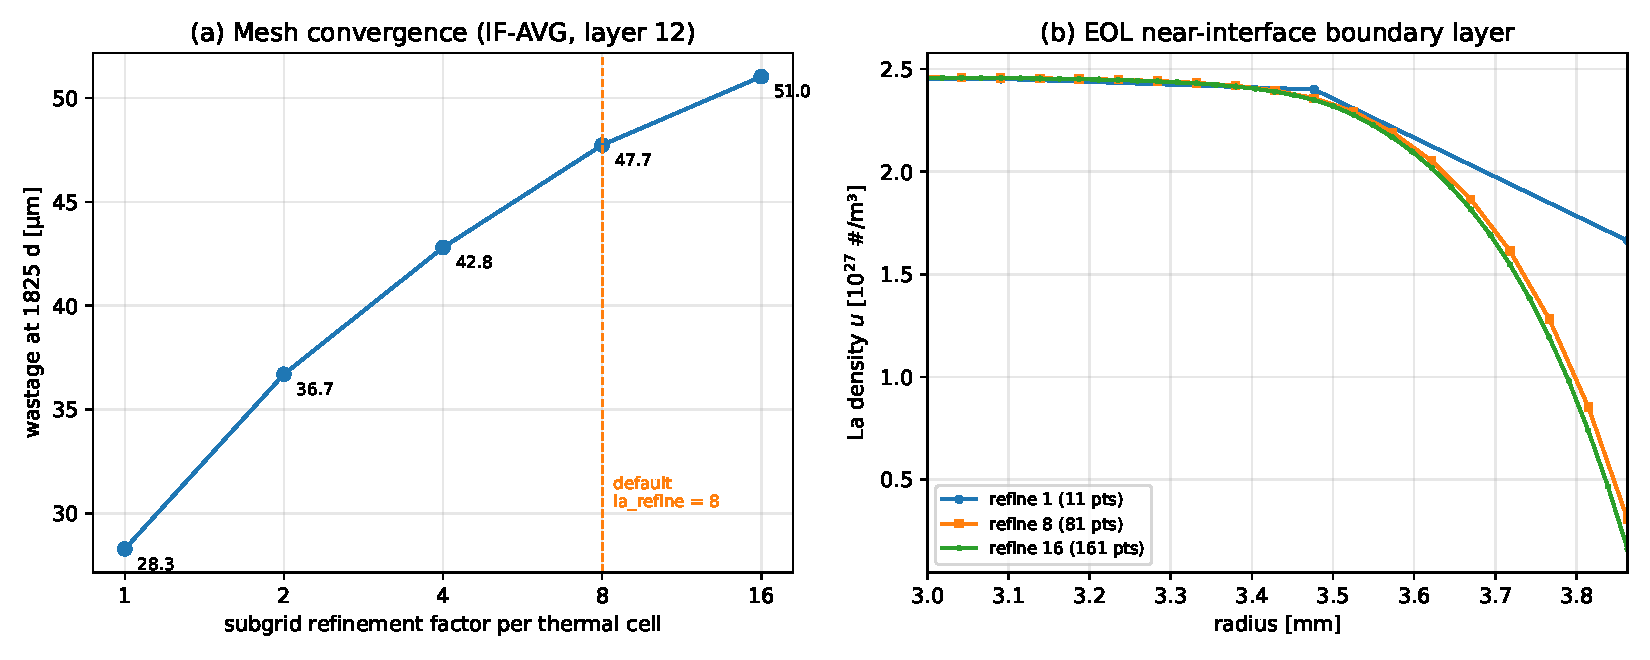
\includegraphics[width=0.95\textwidth]{images/la_mesh_refinement.pdf}
  \caption{LaTracking mesh-refinement study (IF-AVG benchmark, layer 12,
  1825~d): (a)~wastage vs.\ subgrid refinement factor per thermal cell —
  the thermal-grid solve (factor~1) recovers only 55\,\% of the
  $\times16$ reference, the default $\times8$ recovers 93\,\%;
  (b)~end-of-life lanthanide density near the fuel--cladding interface,
  showing the sub-cell boundary layer the coarse grid cannot represent.
  Generated by \texttt{images/make\_la\_mesh\_refinement.py}.}
  \label{fig:la_mesh}
\end{figure}

The contact gating of the sink is
selectable (\texttt{set\_la\_sink\_requires\_contact}): the default follows
the PK model's \texttt{soft}/\texttt{clos} gate, while the MFUEL-faithful
variant keeps the sink active from $t=0$ (transport through the sodium
bond).  The four-decade variation of $D_{La}$
between 800 and 1100~K makes the radial temperature profile the dominant
driver: the sink boundary layer stays confined to the cool outer
millimetre while the hot core remains source-dominated.  MFUEL declares
cladding failure at $\delta \geq 0.5\,t_{clad,0}$; FRED-M-Na streams the
per-layer $\delta$ (HDF5 \texttt{burnup/xwast\_layer}) and per-node $u$
(\texttt{burnup/c\_la}) for operating-limit assessment, with no feedback
onto the stress-strain solution.  See
\texttt{examples/fred\_m\_na/cladding\_wastage\_models/} for a
side-by-side comparison of the two models.

% -------------------------------------
\subsection{Cladding Void Swelling (HT-9)}
\label{sec:clad_swelling}
% -------------------------------------

Fast-neutron irradiation nucleates and grows voids in the HT-9 matrix,
producing a volumetric dilation of the cladding independent of thermal
expansion.  Two models are selectable at run time via
\texttt{set\_clad\_swelling\_model} (enum \texttt{CladSwellingModel},
implemented in \texttt{FredMNaCladSwelling.hpp}; \texttt{Cswel.for}'s
\texttt{icswel} flag in legacy) and are disabled by default (opt-in, since
this is new capability with no existing script depending on it):

\begin{itemize}
\item \texttt{Hofmann} (default): Hofmann (1985) void-swelling correlation
      \texttt{icswel=1}, a closed-form S-curve function of cumulative fast
      fluence, evaluated per clad node at that node's own temperature.
\item \texttt{SAS4A}: SAS4A User's Manual piecewise-linear swelling
      \emph{rate}, \texttt{icswel=2} (added Timpano/Daniele, 2024-08-06),
      gated on cladding dose and evaluated once at the cladding mid-wall
      temperature.
\end{itemize}

Both models consume the same SAS-derived fast-neutron fluence/dose
bookkeeping (\texttt{Baseir.for}):

\begin{equation}
  \dot{\phi} = q_l \, f_{ltpow} \times 10^{-26}\ \ [10^{22}\,\mathrm{n/cm^2/s}],
  \qquad q_l = q'''\,\pi\,(r_{fo0}^2 - r_{fi0}^2),
  \label{eq:sas_flux}
\end{equation}
\begin{equation}
  \nu(t) = \int_0^t \dot\phi\,\mathrm{d}\tau\ \ [10^{22}\,\mathrm{n/cm^2}],
  \qquad
  D_{dpa}(t) = \int_0^t \dot\phi\,D_{conv}\,\mathrm{d}\tau\ \ [\mathrm{dpa}],
  \label{eq:sas_dose}
\end{equation}

where $f_{ltpow}$ (fast-flux-to-linear-power ratio) and $D_{conv}$
(fluence$\to$dose conversion) are \emph{case-specific neutronics
calibration constants}, not universal physical constants: the defaults
($f_{ltpow} = 6.13209\times10^{14}$, $D_{conv} = 4.0$) are Timpano's
Serpent fit and SAS User's Manual value for the Inner-Fuel-Average pin
position (Superphenix-type spectrum) respectively, overridable via
\texttt{set\_fast\_flux\_calibration}.

\subsubsection{Hofmann (1985) void-swelling correlation}

\begin{equation}
  \frac{\Delta V}{V_0} = S_0 + D, \qquad
  S_0 = 0.01\,R\left[\nu + \frac{1}{\alpha}\ln\!
        \left(\frac{1+\exp[\alpha(\tau-\nu)]}{1+\exp(\alpha\tau)}\right)\right],
  \qquad
  D = (0.01)(0.15)\bigl[1-\exp(-0.10\,\nu)\bigr],
  \label{eq:hofmann_swelling}
\end{equation}
\begin{equation}
  R = 0.085\,\exp\!\left[-1\times10^{-4}(T_C - 400)^2\right],
  \qquad \alpha = 0.75,\quad \tau = 14.2,
  \label{eq:hofmann_R}
\end{equation}

with $T_C$ the clad node temperature in \textdegree C and $\nu$ the
cumulative fluence from Eq.~\eqref{eq:sas_dose} (in the same
$10^{22}$~n/cm$^2$ units the correlation was fit in --- note that, unlike
the historical Bison-manual fluence tracker retained in the output log for
reference only, both swelling models consume this one SAS-derived $\nu$).
$S_0$ is the void-formation term (a logistic incubation-then-growth curve
in fluence) and $D$ the solid-state-reaction term.  The linear (isotropic
$\Delta V/3$) strain applied per clad node is
$\varepsilon_{cs} = (\Delta V/V_0)/3$.

\subsubsection{SAS4A piecewise-linear model}

\begin{equation}
  \dot\varepsilon_{sw,HT9} = \begin{cases}
    0 & D_{dpa} < 100 \\[4pt]
    c(T)\;\dot\phi\,D_{conv} & D_{dpa} \geq 100
  \end{cases}
  \label{eq:sas_swelling}
\end{equation}

\begin{center}
\begin{tabular}{ll}
\toprule
$T$ range [K] & coefficient $c(T)$ [linear interpolation] \\
\midrule
$T \leq 673$        & $8.33\times10^{-5} \to 1.0\times10^{-4}$ \ (breakpoints 623/673) \\
$673 < T \leq 723$  & $1.0\times10^{-4} \to 8.33\times10^{-5}$ \\
$723 < T \leq 773$  & $8.33\times10^{-5} \to 5.0\times10^{-5}$ \\
$773 < T \leq 823$  & $7.5\times10^{-5} \to 2.5\times10^{-5}$ \\
$823 < T \leq 873$  & $5.0\times10^{-5} \to 1.25\times10^{-5}$ \\
$T > 873$           & $0$ \\
\bottomrule
\end{tabular}
\end{center}

evaluated at the cladding mid-wall temperature
$T_{mid} = \tfrac12(T_{ci} + T_{co})$ and integrated (explicit Euler) into
the isotropic linear strain
$\varepsilon_{cs} \mathrel{+}= \dot\varepsilon_{sw,HT9}/3 \cdot \Delta t$,
broadcast uniformly across all clad nodes (legacy: ``use midwall
temperature if model 2 is selected'').

\paragraph{The 100-dpa onset gate.} Void swelling in irradiated
ferritic-martensitic steels shows an experimentally observed
\emph{incubation dose}: at low damage, point defects (vacancies and
self-interstitials) generated by displacement cascades are efficiently
absorbed by the material's existing sink structure (dislocations,
lath/grain boundaries, precipitate interfaces) without net void
nucleation, so measured swelling is negligible.  Only once the dose
exceeds a threshold --- here 100 dpa, the SAS4A/HT-9 calibration --- does
the sink structure saturate and voids begin nucleating and growing at an
appreciable, roughly steady rate.  The SAS4A model represents this as a
hard step (zero below, piecewise-linear-in-$T$ above); the Hofmann
correlation instead builds the same incubation behaviour into a smooth
logistic term ($S_0$ above), which is why the two models can diverge
substantially in the first few hundred dpa even though both agree that
early-life swelling is negligible.

Neither model reduces $\varepsilon_{cs}$: void swelling is
irreversible, and (as with the wastage and GRSIS models) the gap-contact
ratchet never reopens for U-Pu-Zr, so there is no legacy reset branch to
reproduce here.  The isotropic strain $\varepsilon_{cs}$ is wired into
the clad Hooke's law identically to thermal expansion --- added with
coefficient $+1$ to the hoop, radial, and axial equations alike (unlike
creep, which is deviatoric and uses the standard $-1/+0.5/+0.5$ split).
FRED-M-Na streams $\varepsilon_{cs}$, $\nu$, and $D_{dpa}$ per layer/node
(HDF5 \texttt{swelling/ecs}, \texttt{swelling/neuflue2},
\texttt{swelling/dose}).  See
\texttt{examples/fred\_m\_na/cladding\_swelling\_models/} for a
side-by-side Hofmann-vs-SAS4A comparison validated against the legacy
Fortran reference.

% -------------------------------------
\subsection{HT-9 Cladding Material}
\label{sec:ht9}
% -------------------------------------

The HT-9 ferritic-martensitic steel correlations for thermal conductivity, heat capacity, thermal expansion, Young's modulus, and Poisson ratio are taken from Karahan (2009) \cite{karahan2009} and ported from \texttt{Clanth.for} in the reference Fortran code \cite{timpanoFredM}. No irradiation creep is currently modelled for HT-9.

% -------------------------------------
\subsection{Sodium Sub-Channel Coolant Model}
\label{sec:subchannel_mna}
% -------------------------------------

FRED-M-Na implements a one-dimensional sub-channel model to compute the local bulk coolant temperature and the cladding-to-coolant HTC axially from inlet conditions.  This enables the Robin boundary condition~\eqref{eq:robin_bc} to be applied without a separate T-H code. The last axial coolant temperature of the subchannel is also used to update the gas plenum temperature, which has a significant effect on the gas plenum pressure.

\subsubsection{Axial Coolant Energy Balance}

The coolant temperature rise from the rod inlet ($j=0$) to each axial layer $j$ is determined by a steady-state energy balance on the sub-channel control volume of layer $j$:

\begin{equation}
  \dot{m}\,c_{p,Na}(T_{co,j})\,\bigl(T_{co,j} - T_{co,j-1}\bigr)
  = q''_{co,j}\cdot 2\pi r_{co}\,\Delta z_j
  \label{eq:subchannel_energy}
\end{equation}

where
\begin{itemize}
\item $\dot{m}$ [kg/s] is the sub-channel mass flow rate,
\item $c_{p,Na}(T)$ [J/(kg\,K)] is the isobaric heat capacity of liquid sodium,
\item $T_{co,j}$ [K] is the bulk coolant temperature at the outlet of layer $j$ (inlet of layer $j+1$),
\item $q''_{co,j} = h_{cool,j}\,(T_{out,j} - T_{co,j})$ [W/m$^2$] is the cladding outer surface heat flux evaluated at the current outer cladding temperature $T_{out,j} \equiv T_{n_f+n_c-1,j}$, and
\item $\Delta z_j$ [m] is the layer height.
\end{itemize}

The equation is solved sequentially from $j=0$ to $j=n_z-1$, with $T_{co,-1} = T_{inlet}$ prescribed by the user.

\paragraph{Sodium thermophysical properties.} Liquid sodium density, specific heat, and thermal conductivity are evaluated from empirical correlations as functions of temperature. The sodium thermal conductivity is used internally for the gap conductance model (Section~\ref{sec:gap_mna}).

\subsubsection{Cladding-to-Coolant HTC Correlations}

The sub-channel HTC $h_{cool}$ [W/(m$^2$\,K)] is computed from a Nusselt number correlation for sodium-cooled pin bundles:
\begin{equation}
  h_{cool} = \frac{k_{Na}(T_{co})\,\mathrm{Nu}}{d_h}
  \label{eq:htc_def}
\end{equation}
where $k_{Na}$ is the sodium thermal conductivity, $\mathrm{Nu}$ the Nusselt number, and $d_h$ the hydraulic diameter of the sub-channel.

Two correlations are available.

\paragraph{Mikityuk (2009) correlation.}
\begin{equation}
  \mathrm{Nu}_{Mik} = 0.047\!\left(1 - e^{-3.8(P/D - 1)}\right)
                      \!\left(\mathrm{Pe}^{0.77} + 250\right)
  \label{eq:nu_mikityuk}
\end{equation}
valid for $1.1 \leq P/D \leq 1.95$ and $30 \leq \mathrm{Pe} \leq 5000$ \cite{mikityuk2009}, where $P/D$ is the pin pitch-to-diameter ratio and $\mathrm{Pe} = \mathrm{Re}\,\mathrm{Pr}$ the Péclet number.

\paragraph{Subbotin (Ushakov) correlation.}
\begin{equation}
  \mathrm{Nu}_{Sub} = 7.55\,\frac{P}{D} - 20\left(\frac{P}{D}\right)^{-13}
                      + \frac{3.67}{90}\,\mathrm{Pe}^{0.56 + 0.19\,P/D}
  \label{eq:nu_subbotin}
\end{equation}
\cite{subbotin1962}.  The Subbotin correlation was used in the legacy FRED-M reference code (option \texttt{COOL\_HTC 2}).

\paragraph{Péclet number.} The Péclet number for sodium flow is:
\begin{equation}
  \mathrm{Pe} = \frac{\dot{m}\,d_h}{A_{ch}\,\rho_{Na}}\,
                \frac{\rho_{Na}\,c_{p,Na}}{k_{Na}}
              = \frac{\dot{m}\,c_{p,Na}\,d_h}{A_{ch}\,k_{Na}}
  \label{eq:peclet}
\end{equation}
where $A_{ch}$ [m$^2$] is the sub-channel flow area.

\printbibliography[heading=subbibliography,title={References}]
\end{refsection}
